%=====================================================
%====== If you are new to LaTeX, this website ========
%======     will be your new best friend:     ========
%======   http://en.wikibooks.org/wiki/LaTeX  ========
%======   Template created by Jonathan Blair  ========
%=====================================================



%=====================================================
%============ Controls ===============================
%=====================================================

%\documentclass[12pt,letterpaper,onecolumn]{article}
\documentclass[11pt,letterpaper,onecolumn]{article}
%\documentclass[10pt,letterpaper,onecolumn]{article}  % not recommended
%\documentclass[12pt,letterpaper,twocolumn]{article}
%\documentclass[11pt,letterpaper,twocolumn]{article}
%\documentclass[10pt,letterpaper,twocolumn]{article}


\usepackage{amsmath}
\usepackage{graphicx}
\usepackage{url}
\usepackage{textgreek}
\usepackage{float}
\usepackage{booktabs}
\usepackage{subcaption}
%\graphicspath{{path-to-folder-containing-necessary-graphics}{other folder as necessary}}


%=====================================================
%============ \begin{document} =======================
%=====================================================

\begin{document}

%=====================================================
%============ Title ==================================
%=====================================================

\title{\bf Observation of the Behavior of an Flip-Flop Devices}
%\title{\Large\bf Larger, Bolded Title}

%=====================================================
%============ Author =================================
%=====================================================
\author{
 Jairo Portillo \\*
  \\*
 PHY 338K Electronic Techniques \\* 
 Department of Physics \\*
 The University of Texas at Austin \\*
 Austin, TX 78712, USA
}
\date{May 6, 2016}

%\address{The University of Texas, Austin, Texas, 78712}

\maketitle

%=====================================================
%============ Abstract ===============================
%=====================================================

\begin{abstract}

In this lab, we will explore the behavior of a Flip Flop devices. We will review the NAND flip flop and observe properties of JK flip flops. We will confirm the JK flip flop table and observe the behavior of a Jk flip flop counter. 
\end{abstract}

%=====================================================
%============ Body of the article ==========================
%=====================================================

%=====================================================
%============ Section ==================================
%=====================================================

\section{Preperation}

 In order to prepare for this lab, we review the behavior of the NAND Gate flip flop from the previous lab and the JK flip flop. As we already know a NAND Gate follows the Boolean function
$$\text{Not(A and B)}$$
and produces the folowwing truth table. 
 \begin{table}[H]
\centering
\begin{tabular}{|c|c|c|}
 \hline
 A & B & F \\\hline
 0 & 0 & 1 \\
 0 & 1 & 1 \\
 1 & 0 & 1 \\
 1 & 1 & 0 \\
  \hline
\end{tabular}
\caption{NAND Gate Behavior}
\label{tab:NAND}
\end{table}
 
 For the NAND flip flop, we know the configuration is
 
 \begin{figure}[H]
    \centering
    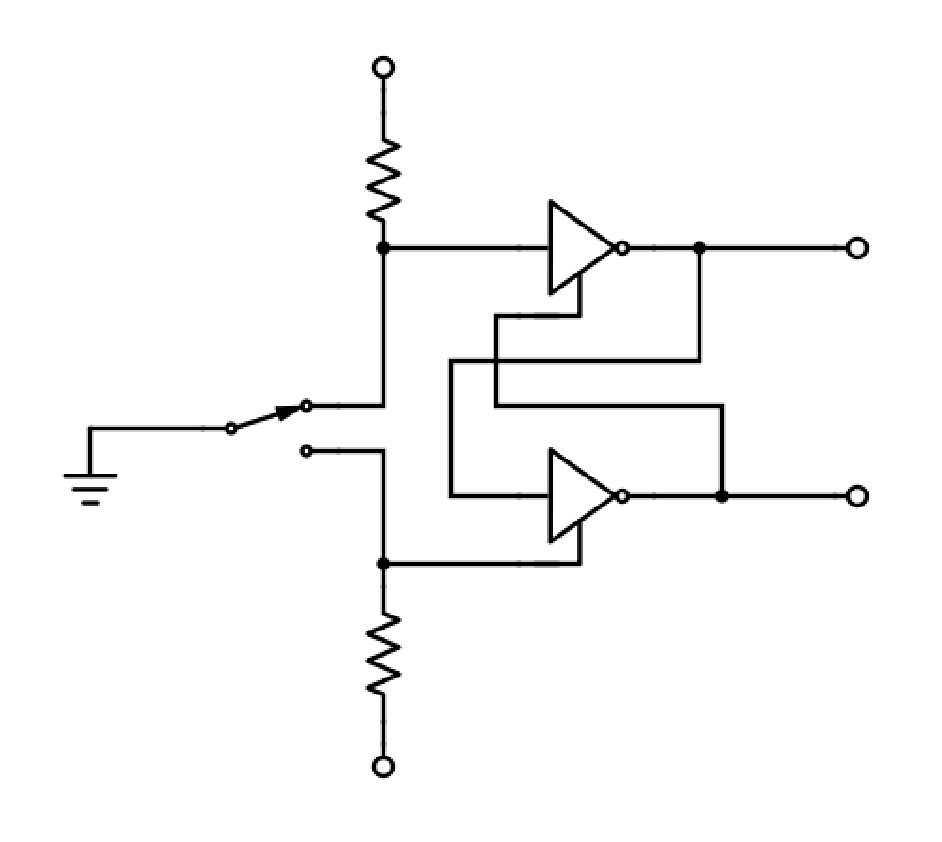
\includegraphics[scale = .5]{cross1.pdf}
    \caption{A Flip Flop NAND with resistors.}
    \label{fig:data2}
\end{figure} 

with the truth table being

 \begin{table}[H]
\centering
\begin{tabular}{|c|c|c|c|}
 \hline
 S & R & $Q_1$ & $Q_2$ \\\hline
 0 & 0 & ? & ?\\
 0 & 1 & 1 & 0 \\
 1 & 0 & 0 & 1 \\
 1 & 1 & $\emptyset$ & $\emptyset$ \\
  \hline
\end{tabular}
\caption{NAND Gate Behavior}
\label{tab:NAND1}
\end{table}
 
 When both inputs are grounded there is no output as it is not an acceptable state and whenever one is grounded and the other is triggered one of the outputs gives a voltage and does not change until the voltage in the inputs is switched. 
 
\begin{figure}[H]
    \centering
    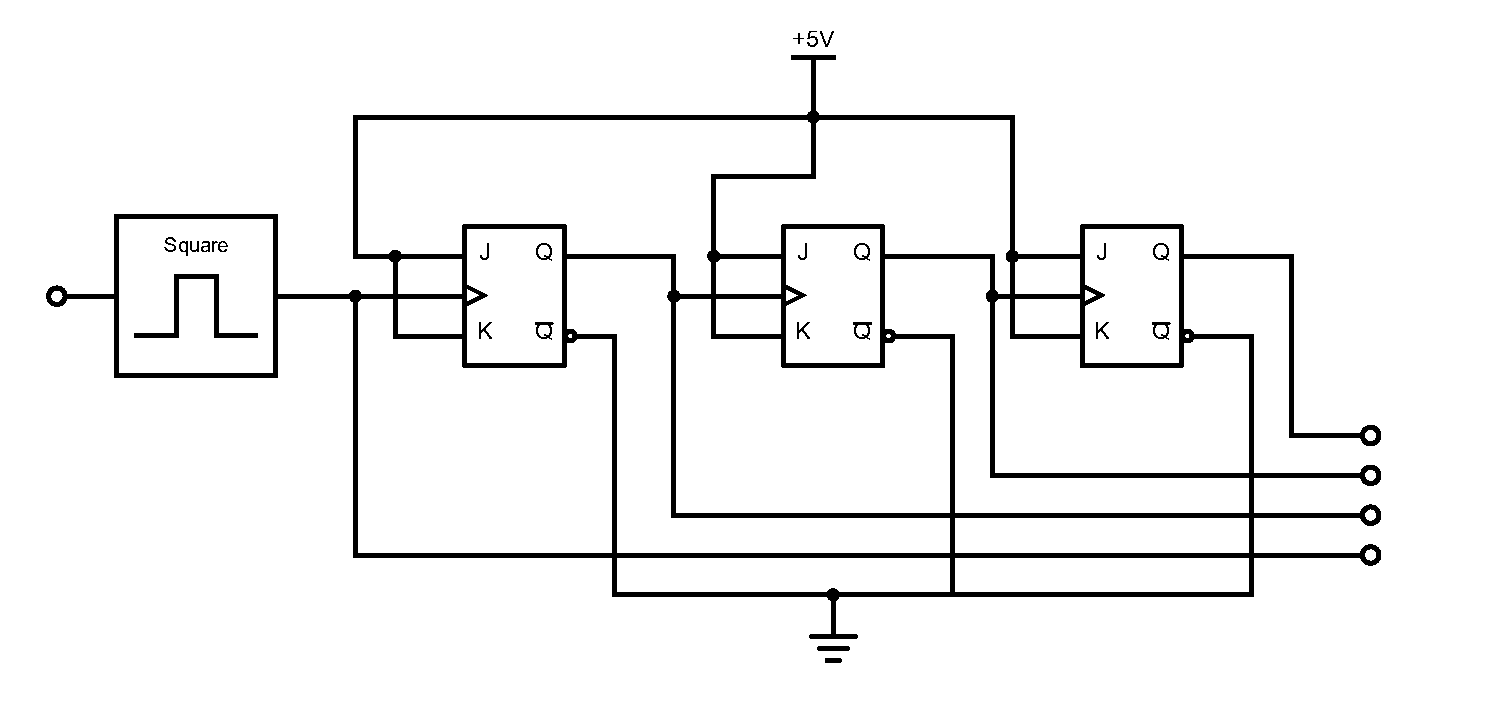
\includegraphics[scale = .6]{flipflop.pdf}
    \caption{JK Flip-Flop Counter}
    \label{fig:my_label}
\end{figure}

The JK flip flop is simply a flip flop gate in a single device rather that using multiple logic gates. It is essentially an integrated circuit of AND gates is a flip flop formation. JK flip flops include a clocked input which can alter the output depending on the state of the inputs when the clocked pulse arrives. The truth table for the JK flip flop is 

 \begin{table}[H]
\centering
\begin{tabular}{|c|c|c|c|}
 \hline
 J & K & $Q_1$ & $Q_2$ \\\hline
 0 & 0 & $\emptyset$ & $\emptyset$\\
 0 & 1 & 1 & 0 \\
 1 & 0 & 0 & 1 \\
 1 & 1 & $0\leftrightarrow 1$ & $0\leftrightarrow1$ \\
  \hline
\end{tabular}
\caption{JK Flip Flop Behavior}
\label{tab:JKff}
\end{table}
 
When there are two inputs, the output is dependent on the clock input thus the outputs may be 1 or 0. The $\emptyset$ means that the output is simply what ever it previously was.

\section{Lab work}

In this lab we simply set up the circuits in Fig 1 and Fig 2. We used 5V for the TRUE input and ground for the FALSE input. For the NAND flip flop gate and JK flip flop gate we observed the results as expected in Table 1 and 2. In order to test the counter each of the output was connected to LEDs as represented by the ports in Fig 2. The LED would respond to the outputs while the LED connected to the oscillator simply oscillated on and off. As the oscilation occured the LED would turn on in sequence as floows.
\begin{table}[]
    \centering
    \begin{tabular}{|c|c|c|c|}
   \hline
 $Q_3$ & $Q_2$ & $Q_1$ & Value\\ \hline
  0 & 0 & 0 & 0\\
  0 & 0 & 1 & 1\\
  0 & 1 & 0 & 2\\
  0 & 1 & 1 & 3\\
  1 & 0 & 0 & 4\\
  1 & 0 & 1 & 5\\
  1 & 1 & 0 & 6\\
  1 & 1 & 1 & 7\\
       
    \hline
    \end{tabular}
    \caption{Caption}
    \label{tab:my_label}
\end{table}

\section{Summary and conclusions}

In this lab, we have reviewed the NAND flip flop and saw how a JK flip flop operates on its own and as a counter. We confirmed the the truth table for the NAND flip flop and JK flip flop. We saw how the JK flip flop counter could count to 7 in binary with the rate at which is counted being dependent on the frequency of the gien input wave. 



%=====================================================
%============ Bibliography  ==============================
%=====================================================



%=====================================================
%============ End ====================================
%=====================================================

\end{document}

%=====================================================
%============ End ====================================
%=====================================================